% =====================================================================
%  Data Mining · SGH · SMMD-ADA   —   Block 4 slide deck
%  Template: Frankfurt + seahorse + miniframes (same as course template)
%
%  Compilation:
%    pdflatex block4.tex   (run twice for the section headline)
%
%  Figures: regenerate with   uv run python lecture_4/make_figures.py
%
%  Speaker-notes display modes (uncomment one):
%    \setbeameroption{hide notes}                          % slides only
%    \setbeameroption{show notes}                          % slides + note pages
%    \setbeameroption{show notes on second screen=right}   % presenter mode
%    \setbeameroption{show only notes}                     % notes printout
% =====================================================================
\documentclass[10pt,aspectratio=169]{beamer}

\usepackage[utf8]{inputenc}
\usepackage[T1]{fontenc}
\usepackage{booktabs}
\usepackage{array}
\usepackage{multirow}
\usepackage{amsmath,amssymb}
\usepackage{graphicx}
\usepackage{xcolor}
\usepackage{tikz}
\usetikzlibrary{arrows.meta,positioning,shapes.geometric}

% - Theme -
\usetheme{Frankfurt}
\usecolortheme{seahorse}
\useoutertheme{miniframes}
\setbeamertemplate{navigation symbols}{}
\setbeamertemplate{footline}[frame number]

% - Speaker notes -
\setbeameroption{hide notes}
% \setbeameroption{show notes on second screen=right}

% - Colours for figures -
\definecolor{sghblue}{RGB}{0,51,102}

% - Metadata -
\title[Data Mining]{Data Mining}
\subtitle{Block 4 - Clustering \& dimensionality reduction}
\author{Daniel Wlazło}
\institute{SGH Warsaw School of Economics - SMMD-ADA}
\date{27 October 2026}

\begin{document}

% ============================================================
\begin{frame}[plain]
  \begin{center}
    \vspace{1cm}
    {\LARGE\textbf{Data Mining}}\\[0.5cm]
    {\large Block 4 - Clustering \& dimensionality reduction}\\[1.5cm]
    {\large Daniel Wlazło} \\[0.2cm]
    {\small SGH Warsaw School of Economics - SMMD-ADA} \\[0.2cm]
    {\small 27 October 2026}
  \end{center}
\end{frame}

% ============================================================
\begin{frame}{Today, hour by hour}
  \begin{enumerate}
    \item \textbf{Recap} - where the supervised half left us \hfill {\small$\sim$5 min}
    \item \textbf{The unsupervised mindset} - no labels, new rules \hfill {\small$\sim$15 min}
    \item \textbf{Distance \& scaling} - the choices before any algorithm \hfill {\small$\sim$20 min}
    \item \textbf{K-means} - and how to choose $k$ \hfill {\small$\sim$35 min}
    \item \textbf{Hierarchical \& DBSCAN} - two other shapes of ``similar'' \hfill {\small$\sim$25 min}
    \item \textbf{PCA} - compressing without a target \hfill {\small$\sim$30 min}
    \item \textbf{Segmentation in practice} - profiling, naming, traps \hfill {\small$\sim$15 min}
    \item \textbf{Lab} - notebook \texttt{04\_clustering\_pca} \hfill {\small$\sim$35 min}
  \end{enumerate}
  \vspace{0.3em}
  \begin{center}\small Breaks roughly every 50 minutes.\end{center}
\end{frame}

% ============================================================
\begin{frame}{Last week in five sentences}
  \begin{enumerate}
    \item Trees turn data into \textbf{rules} and find interactions natively
          - but are too nervous to work alone.
    \item Ensembles manufacture disagreement; every model family has a
          \textbf{leash}, and the U-curve is universal.
    \item Judge by \textbf{CV mean $\pm$ spread}; rankings by
          \textbf{AUC/Gini}; probabilities by \textbf{calibration};
          decisions by \textbf{expected cost}.
    \item \textbf{Leakage} makes models look brilliant because every metric
          is its accomplice.
    \item Complexity must \textbf{earn its keep} - and on the real
          portfolio it did, at every rung of the ladder.
  \end{enumerate}
  \vspace{0.5em}
  \begin{center}
    All of that assumed one thing we are about to lose: \alert{a label}.
  \end{center}
\end{frame}

% ============================================================
\begin{frame}{The map, revisited}
  \small
  \begin{center}
  \begin{tabular}{@{}lp{4.4cm}p{4.6cm}@{}}
    \toprule
    Paradigm & Question & Course status \\
    \midrule
    Supervised & predict a known label & Blocks 2--3 \checkmark{} (returns in 6) \\
    \textbf{Unsupervised} & \alert{find structure, no label} & \textbf{Blocks 4--5 - now} \\
    Reinforcement & act, observe reward & mentioned only \\
    \bottomrule
  \end{tabular}
  \end{center}
  \vspace{0.6em}
  \begin{itemize}\small
    \item Within unsupervised, today covers the two classic families:
          \alert{clustering} (group similar customers) and
          \alert{dimensionality reduction} (compress features).
    \item Block 5 adds the other two: co-occurrence patterns and text.
  \end{itemize}
\end{frame}

% ============================================================
% SECTION: MINDSET
% ============================================================
\section{Mindset}

% ---------------------------------------------------------------
\begin{frame}{What changes when the label disappears}
  \begin{columns}[T]
    \begin{column}{0.5\textwidth}
      \textbf{Supervised (Blocks 2--3)}
      \begin{itemize}\small
        \item ``predict \texttt{default}''
        \item ground truth exists
        \item test set settles arguments
        \item errors have prices
      \end{itemize}
    \end{column}
    \begin{column}{0.5\textwidth}
      \textbf{Unsupervised (Blocks 4--5)}
      \begin{itemize}\small
        \item ``find \alert{structure}''
        \item no ground truth at all
        \item no test set can say ``correct''
        \item usefulness is judged by \alert{decisions it improves}
      \end{itemize}
    \end{column}
  \end{columns}
  \vspace{0.8em}
  \begin{center}
    The dangerous consequence: an unsupervised method \alert{always returns
    an answer} - and nothing in the mathematics tells you whether the
    answer means anything. Scepticism graduates from virtue to method.
  \end{center}
\end{frame}

% ---------------------------------------------------------------
\begin{frame}{Why a lender clusters anyway}
  \begin{itemize}
    \item \textbf{Customer segmentation} - strategy, product design,
          communication tone: ``who are our customers, in four sentences?''
    \item \textbf{Anomaly detection} - customers unlike everyone else are
          interesting: fraud, errors, new markets (Block 1's outlier
          perspective, upgraded).
    \item \textbf{A power tool for EDA} - clusters are hypotheses about
          heterogeneity you didn't know to look for.
    \item \textbf{Compression} - hundreds of correlated features
          $\to$ a few components that feed supervised models (PCA, today).
  \end{itemize}
  \vspace{0.5em}
  \begin{center}\small
    What clustering is \alert{not} for, in a regulated shop: making
    individual credit decisions. Segments inform strategy; the PD model
    prices the person.
  \end{center}
\end{frame}

% ---------------------------------------------------------------
\begin{frame}{The segmentation recipe}
  \begin{enumerate}
    \item \textbf{Representation} - which features describe a customer?
          (application-time rule still applies!)
    \item \textbf{Distance} - what does ``similar'' mean, numerically?
    \item \textbf{Algorithm} - k-means / hierarchical / DBSCAN / \ldots
    \item \textbf{Validation} - internal metrics, stability,
          \alert{business sniff test}
    \item \textbf{Naming} - from statistics to a story the organisation
          can use
  \end{enumerate}
  \vspace{0.6em}
  \begin{center}
    Steps 1--2 decide more than step 3 - as usual, the thinking happens
    \alert{before} the algorithm.
  \end{center}
\end{frame}

% ---------------------------------------------------------------
\begin{frame}{Evaluating without truth: the three substitutes}
  \begin{enumerate}
    \item \textbf{Internal metrics} - do the clusters cohere numerically?
          (inertia, silhouette - today). Necessary, never sufficient.
    \item \textbf{Stability} - does the structure survive reseeding,
          resampling, next quarter's data? The unsupervised cousin of
          cross-validation.
    \item \textbf{External usefulness} - profiled against outcomes held
          \emph{out} of the clustering (default rate per segment), and the
          business sniff test.
  \end{enumerate}
  \vspace{0.6em}
  \begin{center}
    Keep this triad in mind all day - every method we meet will be judged
    by it.
  \end{center}
\end{frame}

% ============================================================
% SECTION: DISTANCE
% ============================================================
\section{Distance}

% ---------------------------------------------------------------
\begin{frame}{Distance is a modelling choice}
  For customers $a, b$ with features $x_{a}, x_{b}$:
  \[
    d_{\text{Euclid}}(a,b) = \sqrt{\textstyle\sum_j (x_{aj} - x_{bj})^2}
    \qquad
    d_{\text{Manhattan}}(a,b) = \textstyle\sum_j |x_{aj} - x_{bj}|
  \]
  \begin{itemize}\small
    \item Euclidean: straight line - the default, sensitive to big
          single-feature gaps.
    \item Manhattan: sum of absolute gaps - more forgiving of one extreme
          coordinate.
    \item Cosine (angle, not length): the text-mining favourite -
          returns in Block 5.
    \item Mixed numeric + categorical data needs care: one-hot distances
          are crude; Gower's coefficient is the classical fix (mention,
          not exam material).
  \end{itemize}
\end{frame}

% ---------------------------------------------------------------
\begin{frame}{Worked example: how far apart are two customers?}
  Three standardised features, two customers:
  \begin{center}\small
  \begin{tabular}{@{}lccc@{}}
    \toprule
     & utilisation (SD) & log limit (SD) & age (SD) \\
    \midrule
    Anna & $+1.2$ & $-0.5$ & $-0.8$ \\
    Bartek & $+0.2$ & $+0.7$ & $-0.6$ \\
    \midrule
    difference & $1.0$ & $-1.2$ & $-0.2$ \\
    \bottomrule
  \end{tabular}
  \end{center}
  \[
    d_{\text{Euclid}} = \sqrt{1.0^2 + 1.2^2 + 0.2^2} = \sqrt{2.48} \approx 1.57
    \qquad
    d_{\text{Manhattan}} = 1.0 + 1.2 + 0.2 = 2.4
  \]
  \begin{itemize}\small
    \item In standardised units, ``1.57'' means: about one-and-a-half
          typical customer-to-customer spreads apart.
    \item Note how the age gap ($0.2$) barely matters under Euclid -
          squaring amplifies the big gaps. That is a \alert{choice} you
          made by picking the metric.
  \end{itemize}
\end{frame}

% ---------------------------------------------------------------
\begin{frame}{Which features deserve a vote?}
  The distance treats every column as one vote about similarity -
  so the feature list \emph{is} the definition of ``similar''.
  \begin{itemize}
    \item \textbf{Application-time rule still applies} - segments built on
          post-outcome fields inherit all of Block 3's leakage pathologies.
    \item \textbf{One concept, one vote} - two utilisation variants let
          utilisation vote twice (the correlation heatmap knows).
    \item \textbf{Business-relevant only} - \texttt{customer\_id} never;
          near-constant columns never (they vote ``everyone is similar'').
    \item \textbf{Keep the target out} - \texttt{default} is reserved for
          \emph{profiling}; clustering on it manufactures fake foresight.
  \end{itemize}
  \vspace{0.4em}
  \begin{center}\small
    Ours today: log limit, age, utilisation, months delayed, payment
    ratio, bill trend - six votes, one concept each. \alert{Sex and
    marriage are excluded from the vote on purpose}: protected traits must
    not define ``similar'', even in strategy work.
  \end{center}
\end{frame}

% ---------------------------------------------------------------
\begin{frame}{Scaling is not optional here}
  \begin{center}
    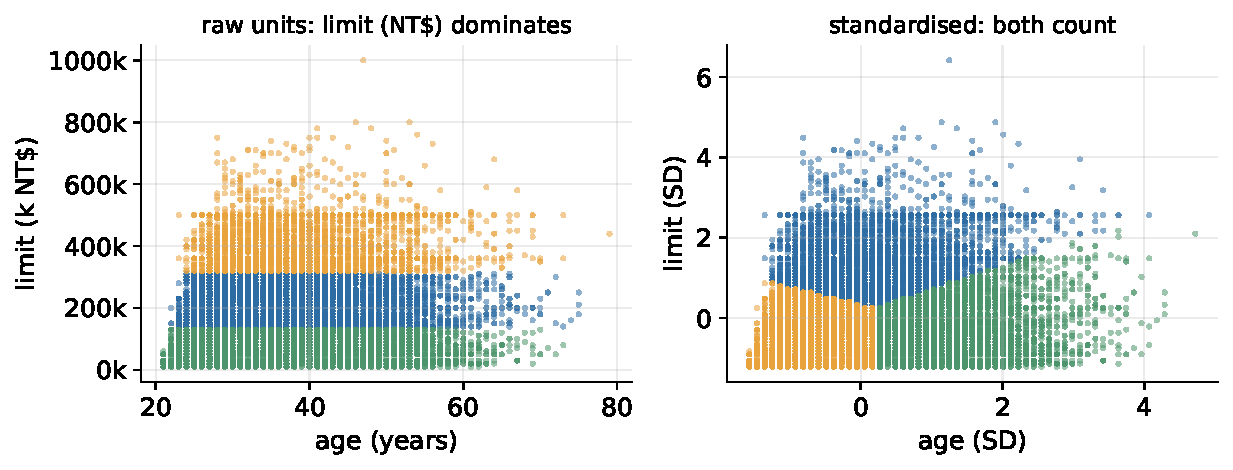
\includegraphics[width=0.86\textwidth]{figures/fig_scaling_matters.pdf}
  \end{center}
  \begin{itemize}\small
    \item Raw units: income (thousands of PLN) dwarfs age (tens of years)
          - distance \alert{is} income, and the ``clusters'' are income
          bands.
    \item Standardise first, always. Trees forgave unscaled features
          (Block 3); \alert{distances never do}.
  \end{itemize}
\end{frame}

% ---------------------------------------------------------------
\begin{frame}{The curse of dimensionality}
  \begin{itemize}
    \item In high dimensions, distances \alert{concentrate}: the nearest and
          the farthest customer become nearly equally far.
    \item Intuition: every extra feature adds a term to the sum; noise
          accumulates until everything is ``average distance'' from
          everything.
    \item Consequences for practice:
      \begin{itemize}\small
        \item cluster on a \alert{curated} feature set, not on everything
              you have;
        \item correlated features silently \alert{double-count} one concept
              (two utilisation variants = utilisation votes twice);
        \item dimensionality reduction (PCA, in an hour) is often the
              opening move.
      \end{itemize}
  \end{itemize}
\end{frame}

% ============================================================
% SECTION: K-MEANS
% ============================================================
\section{K-means}

% ---------------------------------------------------------------
\begin{frame}{K-means in one loop}
  \begin{center}
    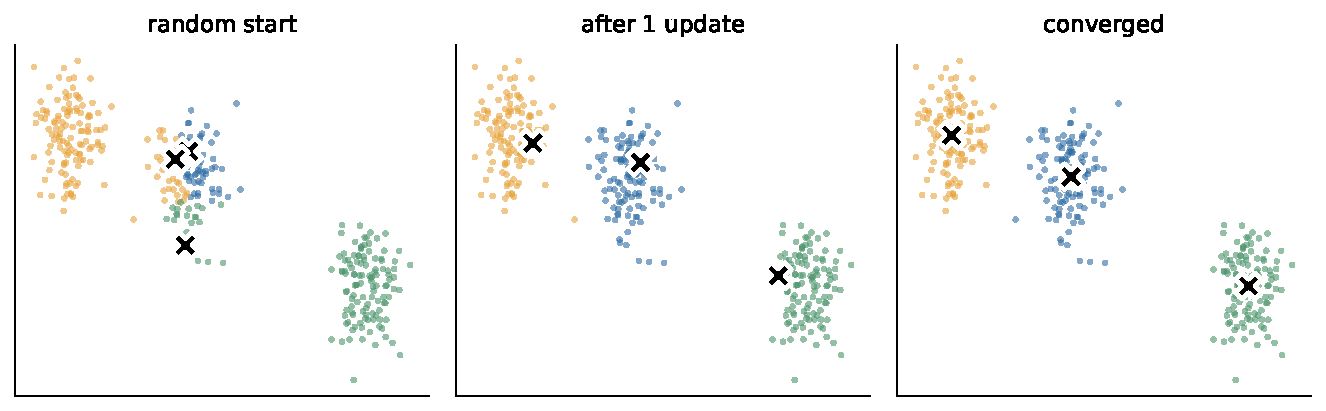
\includegraphics[width=0.9\textwidth]{figures/fig_kmeans_steps.pdf}
  \end{center}
  \begin{itemize}\small
    \item Pick $k$ centres; repeat: \alert{assign} every point to its
          nearest centre, \alert{move} each centre to its points' mean.
    \item Converges quickly - to a \emph{local} optimum that depends on
          the start (hence \texttt{n\_init}: run several starts, keep the
          best; k-means++ picks smarter starts).
  \end{itemize}
\end{frame}

% ---------------------------------------------------------------
\begin{frame}{What k-means optimises}
  \[
    \min_{\text{assignments}}\;
    \sum_{k=1}^{K} \sum_{i \in C_k} \lVert x_i - \mu_k \rVert^2
    \qquad \text{(within-cluster sum of squares, ``inertia'')}
  \]
  \begin{itemize}\small
    \item Each customer belongs to the nearest centre $\Rightarrow$ the
          space is carved into \alert{convex cells} around centroids.
    \item Baked-in assumptions: clusters are roughly \alert{round}, similar
          in size and spread - in the \emph{scaled} space.
    \item Squared distances: sensitive to outliers (a Block 1 reflex should
          fire - inspect before you cluster).
  \end{itemize}
\end{frame}

% ---------------------------------------------------------------
\begin{frame}{K-means on our portfolio}
  \begin{center}
    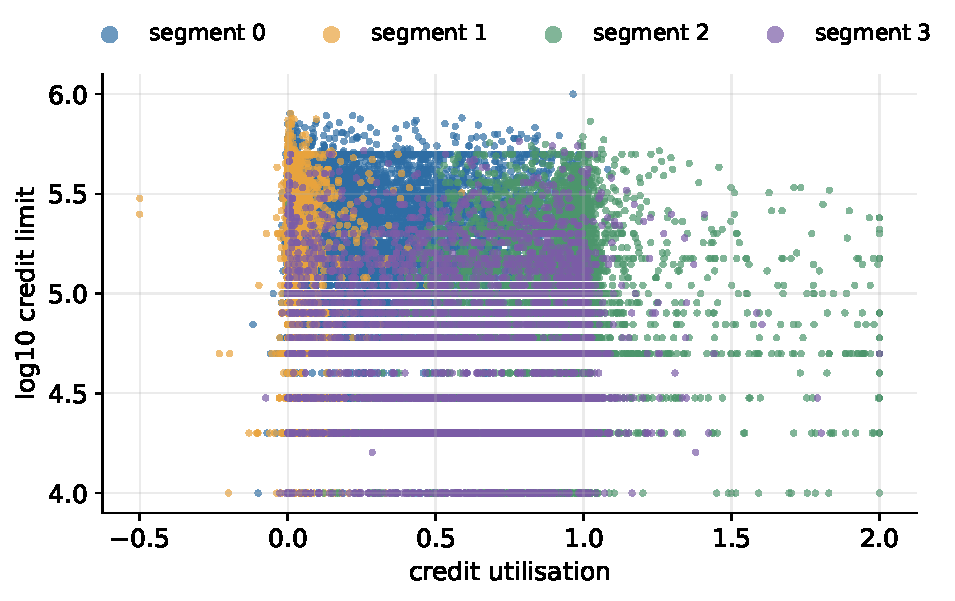
\includegraphics[width=0.45\textwidth]{figures/fig_kmeans_portfolio.pdf}
  \end{center}
  \begin{itemize}\small
    \item Clustered on \alert{six scaled features} (log limit, age,
          utilisation, months delayed, payment ratio, bill trend) - the
          plot shows just one 2-D shadow of it.
    \item No \texttt{default} column in the input - the target is
          reserved for \emph{profiling} the segments later. (Using it
          would smuggle supervision in.)
    \item That dense wall of points at utilisation $\approx 0$?
          \alert{Transactors} - clients who pay in full every month.
          Real structure, visible before any algorithm runs.
  \end{itemize}
\end{frame}

% ---------------------------------------------------------------
\begin{frame}{Practical k-means: starts, speed, reproducibility}
  \begin{itemize}
    \item \textbf{Local optima are real}: a bad random start yields a bad
          partition, silently. \texttt{n\_init=10} runs ten starts and
          keeps the lowest inertia; \alert{k-means++} spreads the initial
          centres out - both are cheap insurance.
    \item \textbf{Reproducibility}: the partition depends on the seed -
          \texttt{random\_state} is part of the segmentation's recipe
          (Block 1's rule, unsupervised edition).
    \item \textbf{Scale}: k-means is fast - millions of rows are fine;
          \texttt{MiniBatchKMeans} trades a little quality for another
          order of magnitude.
    \item \textbf{Outliers}: squared distances make centroids chase extreme
          customers - inspect (or winsorise) first; or use k-medoids,
          which centres on actual customers.
  \end{itemize}
\end{frame}

% ---------------------------------------------------------------
\begin{frame}{Choosing $k$: elbow and silhouette}
  \begin{center}
    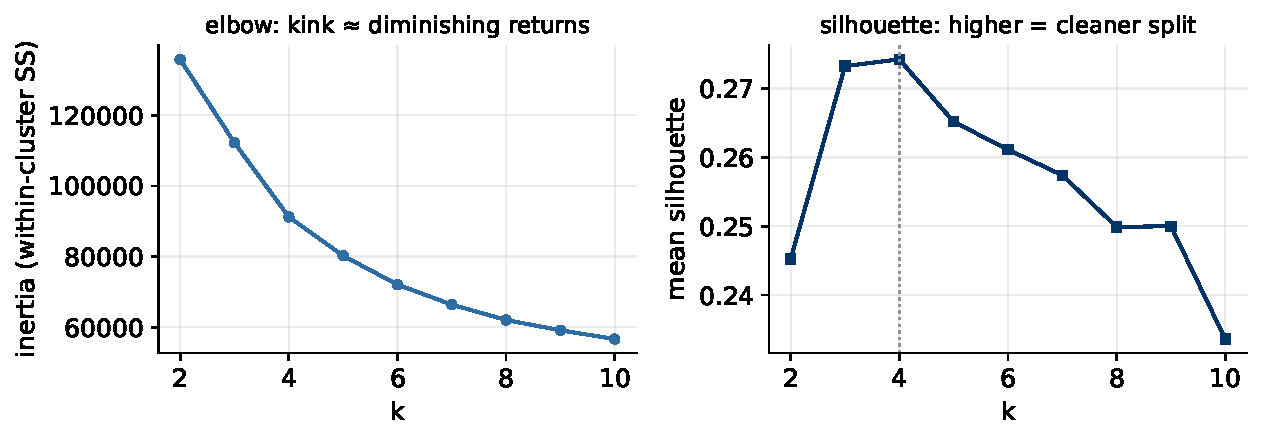
\includegraphics[width=0.92\textwidth]{figures/fig_elbow_silhouette.pdf}
  \end{center}
  \begin{itemize}\small
    \item \textbf{Elbow}: inertia always falls with $k$; look for the kink
          of diminishing returns. Ours: smooth - \alert{no clear kink}.
    \item \textbf{Silhouette} ($-1$ to $1$): how much closer is each
          customer to its own cluster than to the next one? Ours
          \alert{peaks at $k=4$} ($0.27$) - moderate, genuine grouping.
          (Block 1's synthetic cloud scored $0.12$; same diagnostic, both
          verdicts honest.)
  \end{itemize}
\end{frame}

% ---------------------------------------------------------------
\begin{frame}{Silhouette by hand (exam-friendly)}
  For one customer $i$:
  \[
    s_i = \frac{b_i - a_i}{\max(a_i, b_i)}
  \]
  where $a_i$ = mean distance to \emph{own} cluster,
  $b_i$ = mean distance to the \emph{nearest other} cluster.
  \vspace{0.3em}
  \begin{center}\small
  \begin{tabular}{@{}cccl@{}}
    \toprule
    $a_i$ & $b_i$ & $s_i$ & reading \\
    \midrule
    0.4 & 1.6 & $1.2/1.6 = \mathbf{0.75}$ & deep inside its cluster \\
    1.0 & 1.1 & $0.1/1.1 = \mathbf{0.09}$ & sitting on the border \\
    1.5 & 0.9 & $-0.6/1.5 = \mathbf{-0.40}$ & probably mis-assigned \\
    \bottomrule
  \end{tabular}
  \end{center}
  \vspace{0.4em}
  \begin{itemize}\small
    \item The \emph{mean} silhouette over all customers is the number on
          the previous slide's right panel - our $0.27$ now has a face:
          most customers sit clearly closer to home, with a genuine
          borderland in between.
  \end{itemize}
\end{frame}

% ---------------------------------------------------------------
\begin{frame}{Reading the diagnostics honestly}
  A silhouette of $0.27$ is neither noise nor crystal. What does it mean?
  \begin{itemize}
    \item There \alert{is} real grouping - the transactor wall and the
          delinquent tail are genuine behavioural islands - but the
          groups touch: many customers live near a border.
    \item Contrast with Block 1's synthetic portfolio ($0.12$, one cloud):
          the \alert{same diagnostic} separated the two situations. That
          is what diagnostics are for.
    \item K-means returns exactly $k$ sharp-edged segments \alert{either
          way} - the number, not the picture, tells you how much to
          believe.
  \end{itemize}
  \vspace{0.5em}
  \begin{center}
    The report sentence survives: state $k$, the silhouette, and how firm
    the borders are - \emph{every time}.
  \end{center}
\end{frame}

% ---------------------------------------------------------------
\begin{frame}{Where k-means breaks}
  \begin{center}
    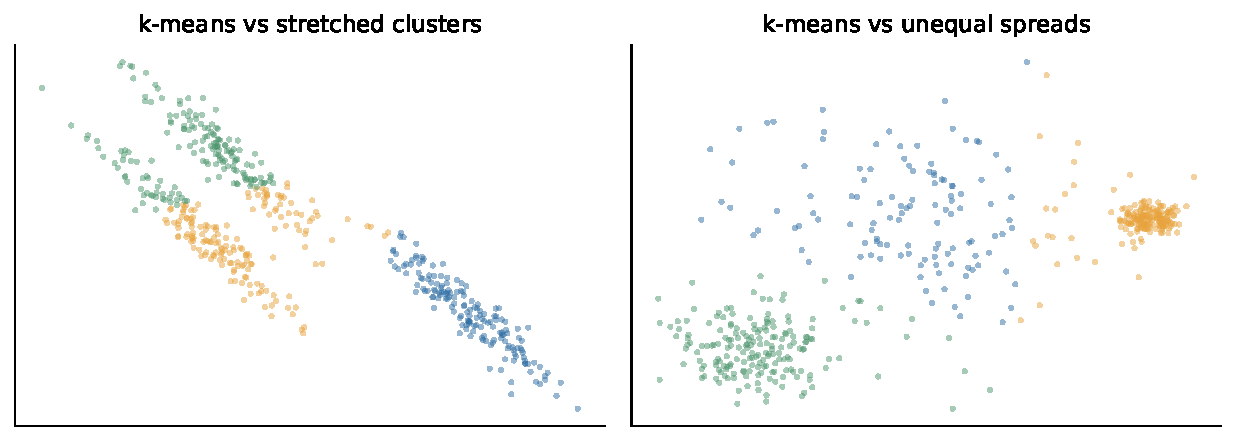
\includegraphics[width=0.86\textwidth]{figures/fig_kmeans_fails.pdf}
  \end{center}
  \begin{itemize}\small
    \item Stretched or unequally spread clusters violate the ``round and
          similar'' assumption - centroids land in the wrong places
          \alert{confidently}.
    \item If the shapes are wrong for the tool, change the tool -
          next section.
  \end{itemize}
\end{frame}

% ============================================================
% SECTION: HIERARCHICAL & DBSCAN
% ============================================================
\section{Hierarchies \& density}

% ---------------------------------------------------------------
\begin{frame}{Agglomerative clustering: merge upward}
  \begin{itemize}
    \item Start: every customer is its own cluster. Repeat: \alert{merge
          the two closest clusters}. Stop when one remains - and record
          the whole merge history.
    \item ``Closest'' between \emph{clusters} needs a definition -
          the \textbf{linkage}:
      \begin{itemize}\small
        \item \textbf{single}: nearest members - chains, snakes;
        \item \textbf{complete}: farthest members - compact, brittle;
        \item \textbf{average}: in between;
        \item \textbf{Ward}: merge that least increases within-cluster
              variance - k-means' cousin, the usual default.
      \end{itemize}
    \item Cost: pairwise distances - fine for thousands, painful for
          millions. (Sample first, or use k-means.)
  \end{itemize}
\end{frame}

% ---------------------------------------------------------------
\begin{frame}{The dendrogram: choose $k$ \emph{after} looking}
  \begin{center}
    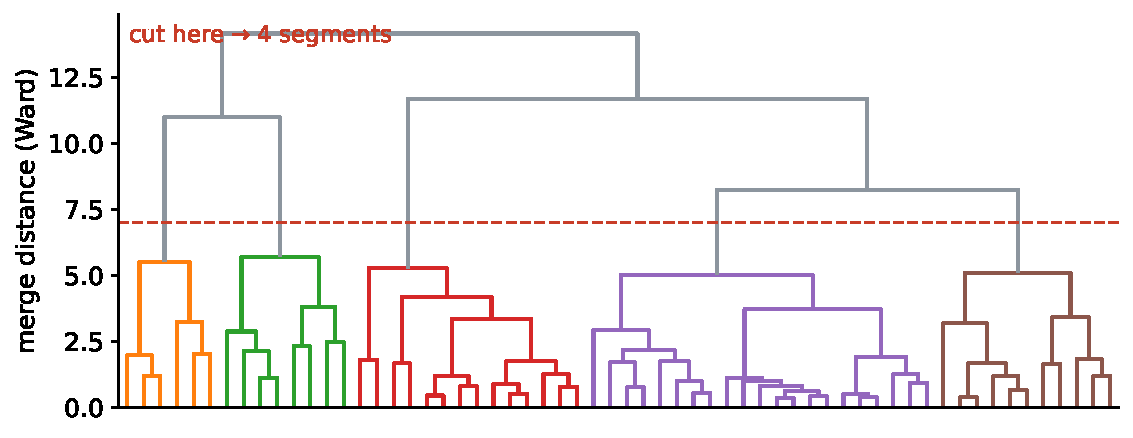
\includegraphics[width=0.88\textwidth]{figures/fig_dendrogram.pdf}
  \end{center}
  \begin{itemize}\small
    \item Height = distance at which two groups merged. Long vertical runs
          = well-separated groups; short ones = arbitrary cuts.
    \item One picture holds \alert{every} $k$ at once - cut where the
          jumps are big. (Ours merges early and often: the weak-structure
          verdict again, from a second witness.)
  \end{itemize}
\end{frame}

% ---------------------------------------------------------------
\begin{frame}{DBSCAN: clusters are dense places}
  \begin{itemize}
    \item Forget centres. A cluster = a region where points are
          \alert{packed}: core points (many neighbours within
          $\varepsilon$), their reachable friends - and everything else
          is \alert{noise}.
    \item Two knobs: $\varepsilon$ (how near is near) and
          \texttt{min\_samples} (how many make ``dense'').
    \item Three superpowers: finds \alert{any shape}; decides the number of
          clusters itself; and \alert{labels outliers} instead of forcing
          them into a segment.
    \item The price: knobs are touchy, and one global density - clusters
          of very different densities confuse it.
  \end{itemize}
  \vspace{0.4em}
  \begin{center}\small
    Fraud-detection perspective: DBSCAN's ``noise'' bucket is sometimes
    the entire deliverable.
  \end{center}
\end{frame}

% ---------------------------------------------------------------
\begin{frame}{Choosing $\varepsilon$: the k-distance elbow}
  \begin{itemize}
    \item DBSCAN's $\varepsilon$ has its own diagnostic: for every point,
          compute the distance to its $k$-th nearest neighbour
          ($k = \texttt{min\_samples}$); sort descending; plot.
    \item The curve falls steeply through sparse space, then flattens where
          density begins - \alert{the knee is your $\varepsilon$}.
    \item Same philosophy as the elbow and the scree plot: let the data
          show its diminishing returns, cut there, and admit it is a
          judgement call.
  \end{itemize}
  \vspace{0.5em}
  \begin{center}\small
    If no knee exists, densities vary too much for one global
    $\varepsilon$ - consider HDBSCAN (hierarchical densities; mention
    only).
  \end{center}
\end{frame}

% ---------------------------------------------------------------
\begin{frame}{Soft memberships: Gaussian mixtures (a mention)}
  \begin{itemize}
    \item K-means answers ``which segment?''; a \alert{Gaussian mixture
          model} answers ``\emph{with what probabilities}?'' - every
          customer gets a membership vector, e.g.\ 70/25/5/0.
    \item Fitted by expectation--maximisation; k-means is the hard-edged
          special case (round, equal clusters, 0/1 memberships).
    \item Why credit likes it: borderline customers \emph{are} the
          interesting ones, and a 55/45 split says ``borderline'' out loud
          - where k-means would silently pick a side.
    \item Same hygiene: scale first, choose components by BIC (its
          information-criterion cousin of the elbow), check stability.
  \end{itemize}
  \vspace{0.4em}
  \begin{center}\small
    sklearn: \texttt{GaussianMixture} - notebook extras.
  \end{center}
\end{frame}

% ---------------------------------------------------------------
\begin{frame}{Shapes k-means cannot see}
  \begin{center}
    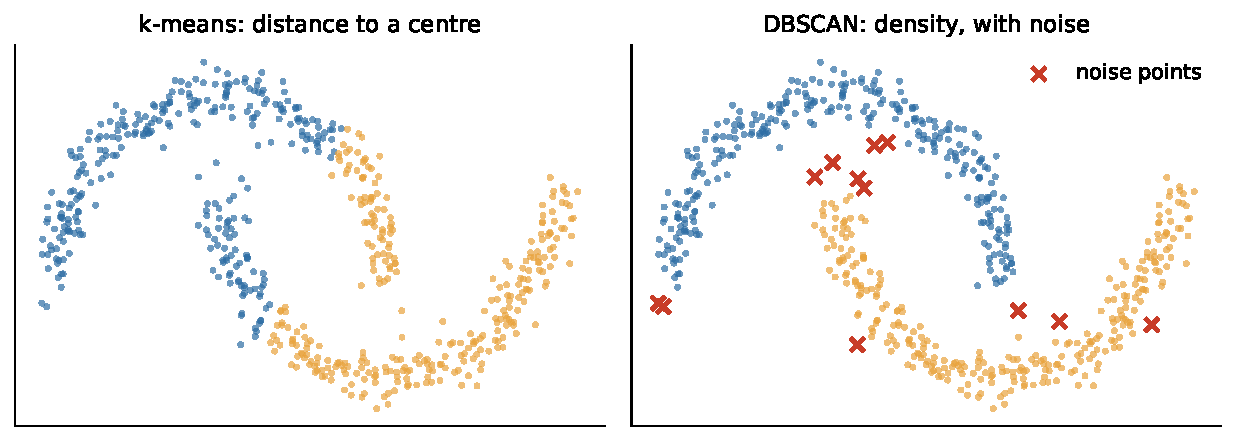
\includegraphics[width=0.86\textwidth]{figures/fig_dbscan_vs_kmeans.pdf}
  \end{center}
  \begin{itemize}\small
    \item Two crescents: k-means slices them with a line (it must -
          convex cells); DBSCAN traces the density and quarantines the
          stragglers as noise.
    \item Crescents are rare in credit; the lesson is general:
          \alert{the algorithm's assumptions decide what it can find}.
  \end{itemize}
\end{frame}

% ---------------------------------------------------------------
\begin{frame}{Choosing the clustering tool}
  \small
  \begin{center}
  \begin{tabular}{@{}llll@{}}
    \toprule
     & k-means & hierarchical & DBSCAN \\
    \midrule
    Cluster shape & round, convex & any (linkage-dep.) & any dense shape \\
    Chooses \#clusters? & no ($k$ input) & after (dendrogram) & yes \\
    Outlier handling & forces them in & forces them in & \alert{noise label} \\
    Scales to millions & yes & no (pairwise) & middling \\
    Randomness & init-dependent & none & none \\
    First pick when & segments wanted & structure unknown & anomalies wanted \\
    \bottomrule
  \end{tabular}
  \end{center}
  \vspace{0.5em}
  \begin{center}
    All three agree on one thing: \alert{scale your features first}.
  \end{center}
\end{frame}

% ============================================================
% SECTION: PCA
% ============================================================
\section{PCA}

% ---------------------------------------------------------------
\begin{frame}{Why compress at all?}
  \begin{itemize}
    \item \textbf{See} - humans plot in 2-D; portfolios live in 20-D.
          A faithful shadow beats twenty histograms.
    \item \textbf{Fight the curse} - fewer, decorrelated dimensions make
          distances meaningful again.
    \item \textbf{De-duplicate} - correlated features (Block 1's heatmap)
          carry one concept several times; components carry it once.
    \item \textbf{Feed models} - components can replace dozens of raw
          features in a supervised model (with a price: interpretability).
  \end{itemize}
  \vspace{0.5em}
  \begin{center}
    The workhorse: \alert{principal component analysis} - linear,
    fast, half a century of service.
  \end{center}
\end{frame}

% ---------------------------------------------------------------
\begin{frame}{PCA: directions of maximal variance}
  \begin{columns}[T]
    \begin{column}{0.5\textwidth}
      \begin{center}
        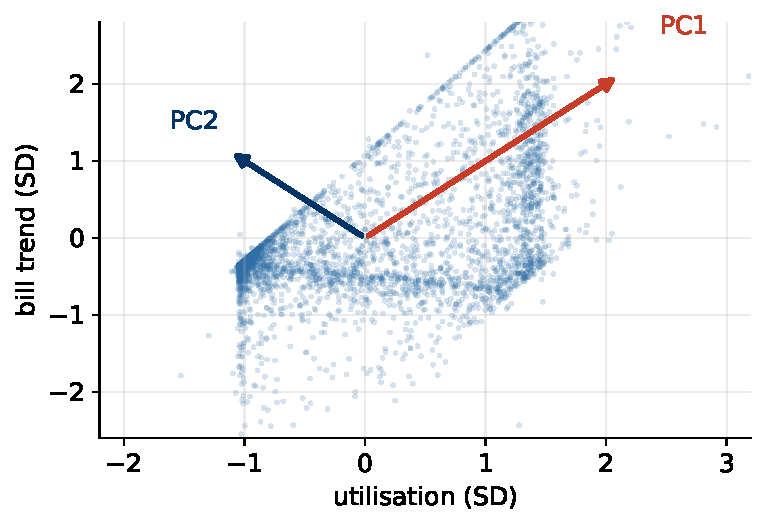
\includegraphics[width=0.9\linewidth]{figures/fig_pca_arrows.pdf}
      \end{center}
    \end{column}
    \begin{column}{0.48\textwidth}
      \vspace{0.6em}
      \begin{itemize}\small
        \item PC1 = the direction along which customers \alert{differ most};
              PC2 = the most-varying direction \emph{perpendicular} to it;
              and so on.
        \item Here: income and savings co-vary (Block 1), so PC1 is their
              shared ``affluence'' axis; PC2 is what's left.
        \item Each customer's \alert{score} on a component = their
              coordinate along that arrow. New features, built from old.
      \end{itemize}
    \end{column}
  \end{columns}
\end{frame}

% ---------------------------------------------------------------
\begin{frame}{The machinery, in one breath}
  PC1 solves: find the unit direction with the most variance,
  \[
    \max_{\lVert w \rVert = 1} \; \operatorname{Var}(Xw)
    = \max_{\lVert w \rVert = 1} \; w^{\top} \Sigma \, w
    \qquad \Longrightarrow \qquad \Sigma\, w = \lambda\, w
  \]
  \begin{itemize}
    \item So the components are the \alert{eigenvectors} of the
          correlation matrix $\Sigma$, ordered by their eigenvalues
          $\lambda$ - which \emph{are} the explained variances
          (computed via SVD in practice).
    \item Components are \alert{orthogonal} (uncorrelated by construction)
          - multicollinearity dies here (Block 2's remedy \#3, delivered).
    \item Each component is a \alert{recipe}: a weighted mix of the original
          features. The weights are the \textbf{loadings} - and the key to
          interpretation.
  \end{itemize}
  \vspace{0.5em}
  \begin{center}\small
    That is all the mathematics we need; sklearn:
    \texttt{PCA(n\_components=...)}, \texttt{fit} / \texttt{transform} -
    the transformer API from Block 2.
  \end{center}
\end{frame}

% ---------------------------------------------------------------
\begin{frame}{How many components? The scree plot}
  \begin{center}
    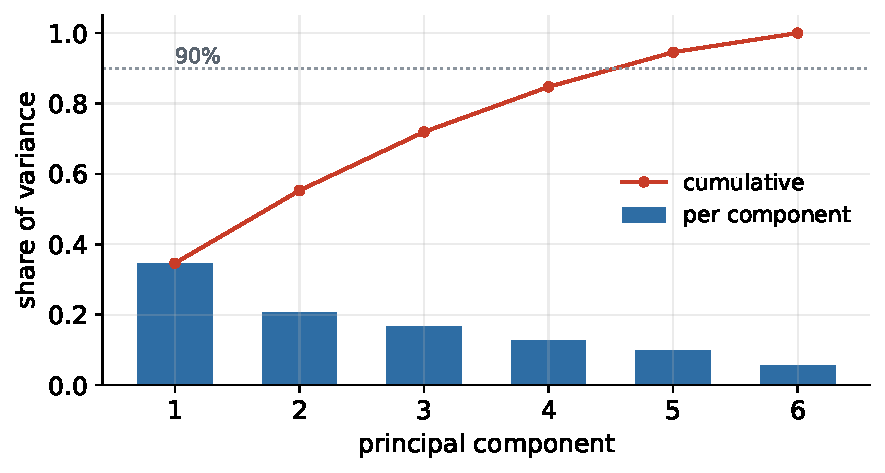
\includegraphics[width=0.64\textwidth]{figures/fig_scree.pdf}
  \end{center}
  \begin{itemize}\small
    \item Our portfolio: PC1 explains 35\%, and 90\% takes \alert{five
          of six} components - moderate compression.
    \item The discount tracks the correlation structure exactly: the
          bill-driven features (utilisation, trend, payment ratio) share an
          axis; age stands alone. PCA compresses redundancy -
          \alert{some redundancy, some discount}.
  \end{itemize}
\end{frame}

% ---------------------------------------------------------------
\begin{frame}{Reading the components: loadings}
  \begin{columns}[T]
    \begin{column}{0.52\textwidth}
      \begin{center}
        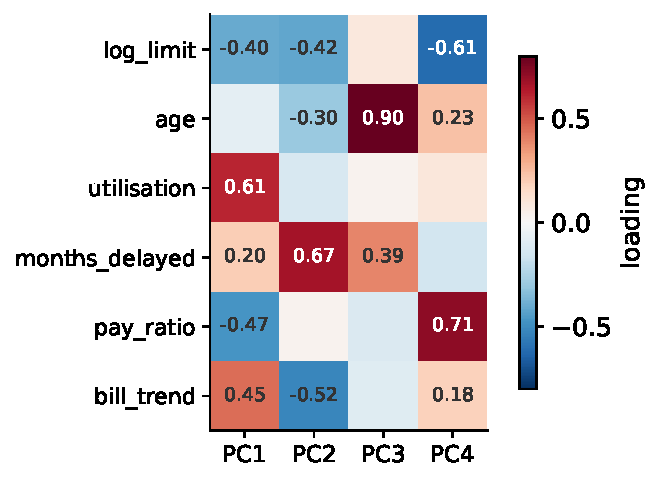
\includegraphics[width=\linewidth]{figures/fig_loadings.pdf}
      \end{center}
    \end{column}
    \begin{column}{0.46\textwidth}
      \vspace{0.6em}
      \begin{itemize}\small
        \item PC1: $+$utilisation, $+$bill trend, $-$payment ratio,
              $-$limit - a \alert{revolving-stress axis}. Nameable!
        \item Naming components is the same craft as naming segments -
              and just as necessary if anyone downstream is to trust them.
        \item A component nobody can name is a feature nobody can defend
              - remember adverse-action reasons.
      \end{itemize}
    \end{column}
  \end{columns}
\end{frame}

% ---------------------------------------------------------------
\begin{frame}{Two views join: segments in PCA coordinates}
  \begin{center}
    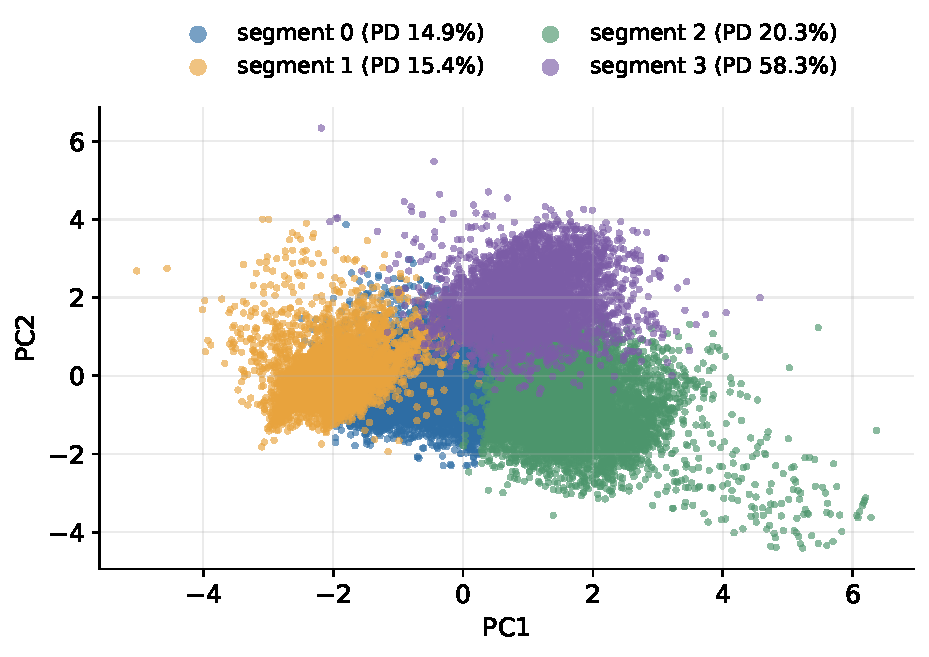
\includegraphics[width=0.48\textwidth]{figures/fig_pca_segments.pdf}
  \end{center}
  \begin{itemize}\small
    \item The 6-D segmentation, shadowed onto the first two components:
          the transactors and the distressed pull visibly apart along
          \alert{PC1, the revolving-stress axis} - the silhouette's
          verdict, drawn.
    \item And the legend carries the punchline: default rates from 15\% to
          \alert{58\%} - structure a strategy team can act on.
  \end{itemize}
\end{frame}

% ---------------------------------------------------------------
\begin{frame}{Another lens: PCA as compression with a receipt}
  \begin{itemize}
    \item Keep $m < p$ components, then \emph{decompress}: rebuild each
          customer from their $m$ scores. The rebuild is imperfect -
          \[
            \text{reconstruction error} \;=\;
            \textstyle\sum_i \lVert x_i - \hat{x}_i \rVert^2
            \;=\; \text{variance you threw away.}
          \]
    \item ``Explained variance 90\% with 5 components'' and
          ``reconstruction loses 10\%'' are the \alert{same sentence} -
          use whichever the audience hears better.
    \item This lens generalises: autoencoders (Block 6's cousins) are
          exactly this idea with nonlinear compress/decompress.
  \end{itemize}
\end{frame}

% ---------------------------------------------------------------
\begin{frame}{Components as features - the leakage-safe way}
  \begin{itemize}
    \item Tempting move: replace the six features with the top components and
          feed them to the Block 3 tournament.
    \item The golden rule follows: PCA has fitted parameters (the loadings)
          - \alert{fit on training data only}, inside the pipeline:
  \end{itemize}
  \vspace{0.3em}
  \begin{center}\small
    \texttt{make\_pipeline(StandardScaler(), PCA(5), LogisticRegression())}
  \end{center}
  \vspace{0.3em}
  \begin{itemize}
    \item Inside cross-validation, the loadings then refit per fold -
          automatically. Outside a pipeline, they silently leak.
    \item Expect no miracle on our portfolio (little redundancy to
          compress) - the point is the \emph{pattern}, which pays off on
          wide, correlated real data.
  \end{itemize}
\end{frame}

% ---------------------------------------------------------------
\begin{frame}{PCA: the fine print}
  \begin{itemize}
    \item \textbf{Scale first} - unscaled, PC1 is simply the
          biggest-variance feature in its raw units (income, again).
    \item \textbf{Variance $\ne$ importance} - PCA never saw the target;
          the risk signal may hide in PC6. Dropping small components can
          drop the signal (check against the supervised task before
          feeding components to models).
    \item \textbf{Linear only} - PCA finds flat directions; curved
          structure survives compression badly.
    \item For \emph{visualisation} of curved structure: t-SNE and UMAP -
          beautiful, nonlinear, and \alert{treacherous}: distances between
          their islands and their densities mean little. Use for pictures,
          never for downstream distances.
  \end{itemize}
\end{frame}

% ============================================================
% SECTION: PRACTICE
% ============================================================
\section{Practice}

% ---------------------------------------------------------------
\begin{frame}{Profiling the segments (ours, $k=4$)}
  \small
  \begin{center}
  \begin{tabular}{@{}lrrrrr@{}}
    \toprule
    Segment & size & limit & util. & delays & \alert{default rate} \\
    \midrule
    0 ``mainstream revolvers'' & 12{,}562 & 174k & 0.20 & 0.3 & 14.9\% \\
    1 ``transactors'' (pay in full) & 4{,}980 & 174k & 0.03 & 0.3 & 15.4\% \\
    2 ``maxed-out borrowers'' & 8{,}576 & 72k & \alert{0.90} & 0.4 & 20.3\% \\
    3 ``\alert{distressed delinquents}'' & 3{,}882 & 54k & 0.60 & \alert{4.2} & \alert{58.3\%} \\
    \bottomrule
  \end{tabular}
  \end{center}
  \vspace{0.4em}
  \begin{itemize}\small
    \item Profile = per-segment means of the \emph{clustering} features
          \alert{plus} outcomes held out of the clustering
          (default rate!) - that is where the business value appears.
    \item Segment 3: four months behind on average, defaulting at
          \alert{58\%} - over $2.5\times$ the portfolio's 22\%. The story
          writes itself - and this is the classic industry quartet
          (transactors / revolvers / maxed-out / distressed), rediscovered
          from scratch by an unsupervised algorithm.
  \end{itemize}
\end{frame}

% ---------------------------------------------------------------
\begin{frame}{From statistics to a story: naming}
  \begin{itemize}
    \item A segment name must be earned by the profile table: short,
          concrete, slightly memorable - ``stretched borrowers'', not
          ``segment~1'' and not ``high-DTI-low-income cluster''.
    \item The test: a product manager should predict the profile
          \emph{from the name alone}.
    \item Dishonest naming is a real failure mode: names imply crisp tribes
          where the data shows a continuum. Pair every name with the
          \alert{soft-boundaries disclaimer} from the silhouette slide.
    \item And write down the recipe (features, scaling, $k$, seed) -
          Block 1's reproducibility rule; next quarter's refresh must
          rebuild \emph{these} segments, not new ones.
  \end{itemize}
\end{frame}

% ---------------------------------------------------------------
\begin{frame}{Is the segmentation stable?}
  With no ground truth, stability is the closest thing to correctness:
  \begin{itemize}
    \item \textbf{Reseed}: different random starts - same segments?
          (Ours: yes, with \texttt{n\_init=10}.)
    \item \textbf{Resample}: cluster on 80\% subsamples - do customers
          stay together? (The unsupervised cousin of CV.)
    \item \textbf{Re-time}: next quarter's data - do the segments
          reappear, or did we photograph noise?
    \item \textbf{Perturb}: drop one feature - does the story survive, or
          did one column dictate everything (the unscaled-income disease in
          disguise)?
  \end{itemize}
  \vspace{0.4em}
  \begin{center}
    Then the strongest validator available: \alert{does the business
    recognise these customers?}
  \end{center}
\end{frame}

% ---------------------------------------------------------------
\begin{frame}{The sobering slide}
  \begin{columns}[T]
    \begin{column}{0.44\textwidth}
      \begin{center}
        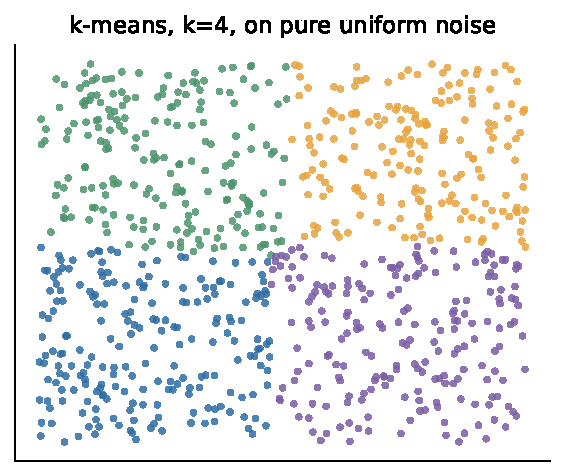
\includegraphics[width=\linewidth]{figures/fig_noise_clusters.pdf}
      \end{center}
    \end{column}
    \begin{column}{0.54\textwidth}
      \vspace{0.8em}
      \begin{itemize}\small
        \item Pure uniform noise. No structure whatsoever. K-means,
              asked for four clusters, \alert{delivers four clusters} -
              tidy, colourful, publishable.
        \item Every clustering deliverable should survive this question:
              \emph{``what would this slide look like on noise?''}
        \item The unsupervised twin of Block 1's ``torturing the data until
              it confesses''.
      \end{itemize}
    \end{column}
  \end{columns}
\end{frame}

% ---------------------------------------------------------------
\begin{frame}{Bonus recipe: k-means as an anomaly detector}
  \begin{itemize}
    \item Every customer has a \alert{distance to their nearest centroid}
          - a one-line outlier score: the further, the stranger.
    \item Shortlist the top 1\% and hand it to investigators - a
          serviceable first fraud screen with zero labels required.
    \item DBSCAN offers the same for free: its \alert{noise bucket} is the
          shortlist.
    \item Block 1's lesson upgraded: outliers are not cleaning waste -
          sometimes the strangest customers \emph{are} the deliverable.
  \end{itemize}
  \vspace{0.5em}
  \begin{center}\small
    Notebook extras: build the shortlist and eyeball its profile against
    the portfolio.
  \end{center}
\end{frame}

% ---------------------------------------------------------------
\begin{frame}{Common segmentation sins}
  \begin{enumerate}
    \item \textbf{Clustering on the target} (or its twins) -
          manufactured foresight; Block 3's leakage in a new costume.
    \item \textbf{Unscaled features} - one column secretly dictates the
          whole segmentation.
    \item \textbf{Too many segments} - fourteen segments no one can
          name is a lookup table, not insight.
    \item \textbf{Hard-boundary storytelling} - crisp names on a
          continuum, without the soft-boundaries sentence.
    \item \textbf{Quarterly renaming} - refitting from scratch each
          quarter and re-deriving ``new'' customer types from seed noise.
    \item \textbf{Skipping the noise question} - never asking what the
          deliverable would look like on shuffled data.
  \end{enumerate}
\end{frame}

% ---------------------------------------------------------------
\begin{frame}{Where segments are allowed to work}
  \begin{itemize}
    \item \textbf{Strategy \& product}: design offers per segment; watch
          segment sizes drift over quarters (a leading indicator of
          portfolio change - ties to Block 3's monitoring).
    \item \textbf{Communication}: tone and channel per segment.
    \item \textbf{As features}: segment membership can enter a supervised
          model - fit the clustering on \alert{training data only}
          (the golden rule follows us everywhere).
    \item \textbf{Not}: as the individual credit decision. Pricing a
          \emph{person} by their \emph{segment} invites both regulatory
          trouble and unfairness - the PD model prices the person
          (and Block 6 returns to fairness properly).
  \end{itemize}
\end{frame}

% ============================================================
% SECTION: LAB
% ============================================================
\section{Lab}

% ---------------------------------------------------------------
\begin{frame}[plain]
  \begin{center}
    \vspace{1.5cm}
    {\LARGE\textbf{Laboratory}}\\[0.6cm]
    {\normalsize Notebook \texttt{04\_clustering\_pca} - laptops out.}
  \end{center}
\end{frame}

% ---------------------------------------------------------------
\begin{frame}{Lab today}
  \begin{columns}[T]
    \begin{column}{0.54\textwidth}
      \textbf{Notebook \texttt{04\_clustering\_pca}}
      \begin{itemize}\small
        \item scale, cluster, and \emph{break} it (unscaled demo)
        \item elbow + silhouette - read weak signals honestly
        \item profile and \alert{name} the $k=4$ segments
        \item dendrogram on a sample; DBSCAN on shapes
        \item PCA: scree, loadings, segments in 2-D
      \end{itemize}
    \end{column}
    \begin{column}{0.44\textwidth}
      \textbf{Done =}
      \begin{itemize}\small
        \item a named segment table with sizes, profiles, and default
              rates
        \item one honest paragraph on how strong the structure really is
      \end{itemize}
      \vspace{0.3em}
      \textbf{Optional extras}
      \begin{itemize}\small
        \item DBSCAN's noise bucket as an anomaly shortlist
        \item components as features in the Block 3 tournament
      \end{itemize}
    \end{column}
  \end{columns}
\end{frame}

% ============================================================
% SECTION: SUMMARY
% ============================================================
\section{Summary}

% ---------------------------------------------------------------
\begin{frame}[plain]
  \begin{center}
    \vspace{1.5cm}
    {\LARGE\textbf{Summary}}\\[0.6cm]
    {\normalsize What to take home from Block 4.}
  \end{center}
\end{frame}

% ---------------------------------------------------------------
\begin{frame}{Block 4 in five sentences}
  \begin{enumerate}
    \item Without labels there is no ``correct'' - only \textbf{useful},
          and usefulness is argued, not measured.
    \item \textbf{Distance is a modelling choice}, and unscaled features
          make it silently for you - always standardise.
    \item K-means carves round cells and \textbf{always answers};
          elbow, silhouette and stability tell you how much to believe it.
    \item Hierarchies show all $k$ at once; \textbf{DBSCAN} finds shapes
          and names outliers - assumptions decide what each tool can see.
    \item \textbf{PCA} compresses redundancy into nameable axes - and
          its discount always equals the redundancy it finds - no more, no less.
  \end{enumerate}
\end{frame}

% ---------------------------------------------------------------
\begin{frame}{Project status \& reminder}
  \begin{itemize}
    \item Three weeks to the presentation (Block 7) - your two model
          families should exist \alert{this week}, however rough, so the
          final fortnight belongs to evaluation and the slides.
    \item If your project uses segmentation: it must arrive with the
          honesty kit - silhouette or stability evidence, the
          soft-boundaries sentence, and named profiles. A pretty scatter
          plot is not a deliverable.
    \item Rubric reminder: interpretation \& recommendation is 15\% -
          segment naming and profiling is precisely that skill.
  \end{itemize}
  \vspace{0.5em}
  \begin{center}\small
    Office-hour priority this week: teams whose topic description flagged
    unresolved data-quality risks.
  \end{center}
\end{frame}

% ---------------------------------------------------------------
\begin{frame}{Exam practice - multiple choice}
  \small
  \textbf{Q1.} Why must features be standardised before k-means?
  \begin{enumerate}[(a)]
    \item k-means only converges on standardised data
    \item features with large units dominate the distance, deciding
          ``similar'' by themselves
    \item standardisation increases the silhouette score
    \item scikit-learn requires it
  \end{enumerate}
  \vspace{0.4em}
  \textbf{Q2.} Your segmentation reports a mean silhouette of 0.27 at $k=4$.
  The honest reading:
  \begin{enumerate}[(a)]
    \item the clustering failed - do not report it
    \item moderate, real-but-touching groups - report the number alongside
          the segments
    \item excellent separation - the segments are firm
    \item $k$ must be increased until silhouette exceeds 0.5
  \end{enumerate}
\end{frame}
% Answer key: Q1 (b) - distance adds feature gaps in raw units; scaling is a
% modelling decision made explicit. Q2 (b) - the honesty clause: state k,
% the silhouette, and how firm the borders are; 0.27 is genuine but soft
% structure, and silhouette-chasing k is not a method.

% ---------------------------------------------------------------
\begin{frame}{Exam practice - open question}
  \begin{block}{In the style of the term-0 exam ($\sim$60\% open questions)}
    A PCA of six behavioural features yields PC1 loadings:
    $+$utilisation, $+$bill\_trend, $-$pay\_ratio, $-$log\_limit.
    Name this component for a product manager and justify the name from the
    loadings. What business action could be indexed to it?
  \end{block}
  \vspace{0.5em}
  \begin{center}\small
    4-6 sentences. A component you can name is a component you can defend.
  \end{center}
\end{frame}
% A good answer: a "revolving stress" axis - customers high on PC1 are
% heavily utilised, with growing bills, repaying small fractions, on small
% limits; customers low on PC1 are the opposite (transactor-like). Actions:
% early-warning monitoring, limit-management or proactive restructuring
% offers ranked by PC1 score. Credit for noting the sign convention is
% arbitrary - the AXIS is real, the direction is a labelling choice.

% ---------------------------------------------------------------
\begin{frame}[plain]
  \begin{center}
    \vspace{1.5cm}
    {\LARGE\textbf{Next week: pattern discovery \& text mining.}}\\[0.6cm]
    {\normalsize What sits in the basket - and what sits in the
    complaints inbox.}
  \end{center}
\end{frame}

% ---------------------------------------------------------------
\begin{frame}{Keep learning - Block 4 reading}
  \begin{itemize}
    \item \textbf{Jain} - \emph{Data Clustering: 50 Years Beyond K-means}
          (Pattern Recognition Letters, 2010) - the survey that puts
          today's toolbox in one story.
    \item \textbf{Jolliffe \& Cadima} - \emph{Principal component analysis:
          a review and recent developments} (Phil.\ Trans.\ R.\ Soc.\ A, 2016).
    \item \textbf{Wattenberg, Vi\'egas \& Johnson} - \emph{How to Use t-SNE
          Effectively} (distill.pub, 2016) - interactive; why 2-D embeddings
          seduce and mislead.
    \item \textbf{scikit-learn User Guide} - \emph{Clustering} section:
          the algorithm-comparison gallery is worth ten lectures.
  \end{itemize}
\end{frame}

\end{document}
